\begin{center}
    \tikzstyle{s} = [rectangle, rounded corners, minimum width=3cm, minimum height=1cm,text centered, draw=black]
    \tikzstyle{arrow} = [thick,->,>=stealth]
    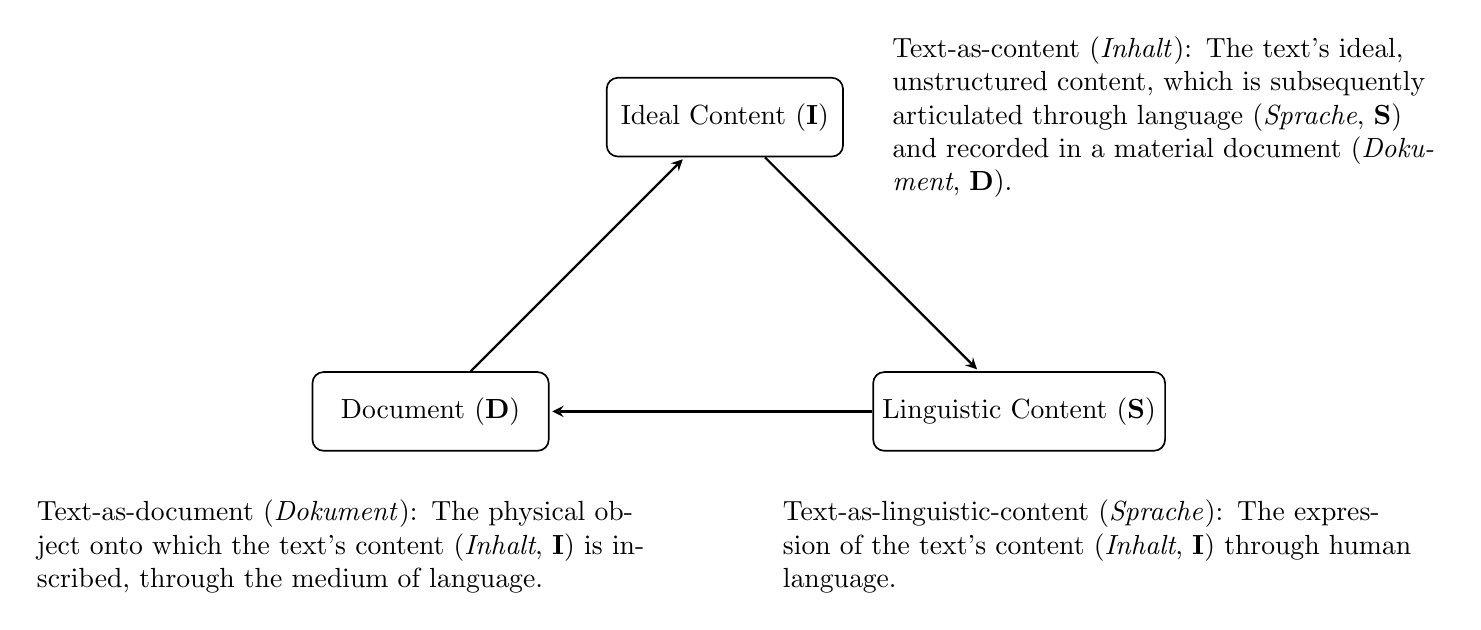
\begin{tikzpicture}[-,shorten >=1pt,auto,node distance=2.8cm,semithick]
    \tikzstyle{every state}=[fill=red,draw=none,text=white]
    \node[s] (D) {Document (\textbf{D})};
    \node[s] (I) [above right of=D, xshift=5em, yshift=5em] {Ideal Content (\textbf{I})};
    \node[s] (S) [below right of=I, xshift=5em, yshift=-5em] {Linguistic Content (\textbf{S})};
    \node [below=1cm,text width=8cm, xshift=1cm] at (S)
    {
    Text-as-linguistic-content (\textit{Sprache}): The expression of the text's content (\textit{Inhalt}, \textbf{I}) through human language.
    };
    \node [below=1cm,text width=8cm, xshift=-1cm] at (D)
    {
    Text-as-document (\textit{Dokument}): The physical object onto which the text's content (\textit{Inhalt}, \textbf{I}) is inscribed, through the medium of language.
    };
    \node [right=2cm,text width=7cm] at (I)
    {
    Text-as-content (\textit{Inhalt}): The text's ideal, unstructured content, which is subsequently articulated through language (\textit{Sprache}, \textbf{S}) and recorded in a material document (\textit{Dokument}, \textbf{D}).
    };
    \draw [arrow] (S) -> (D);
    \draw [arrow] (D) -> (I);
    \draw [arrow] (I) -> (S);
    \end{tikzpicture}
\end{center}